\documentclass[10pt,a4paper]{article}
\usepackage[utf8]{inputenc}
\usepackage[francais]{babel}
\usepackage[T1]{fontenc}
\usepackage{amsmath}
\usepackage{amsfonts}
\usepackage{amssymb}
\usepackage{graphicx}
\usepackage[squaren,Gray]{SIunits} % Physical units rendering
\usepackage{sistyle}
\usepackage[autolanguage]{numprint}
%\usepackage{xfrac}
\usepackage{bm}
\usepackage{color} % Colors in text
\usepackage[version=3]{mhchem} % Chemical reactions

\title{Production d'hydrogène par électrolyse}
\author{Groupe 1254}
\date{10 Novembre 2014}



\begin{document}

\maketitle



Au cours du laboratoire, nous avons fait varier plusieurs paramètres afin de déterminer les meilleurs conditions de production d'hydrogène. Les trois paramètres sont le pH, la température et le courant (en Ampère). Nous avons étudié la vitesse de production d'hydrogène.
\\

Remarque : Certaines mesures manquent ou sont imprécises, nous nous sommes donc inspirées de la solution donnée. \footnote{les graphiques sont tirés du document corrigé fournis sur icampus}

\section{Conditions opératoires de production d'hydrogène}

\subsection{La température}

La température influence la vitesse de réaction : une augmentation de température implique un apport de chaleur qui contribue à diminuer l'énergie à apporter à la réaction (qui est endothermique) et donc l'énergie électrique à apporter sera moindre.



\subsection{Le courant}

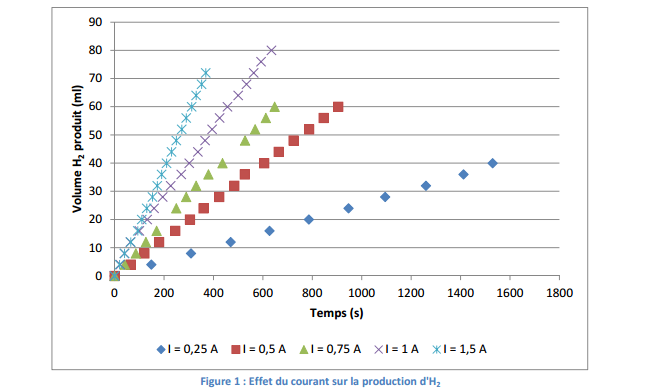
\includegraphics[scale=0.6]{PRODUCTIONHYDRO.png} 
\\
  

Le courant est un paramètre qui influence directement la vitesse de production d'hydrogène. De plus, ces deux grandeurs sont proportionnelles, la production d'hydrogène est donc linéaire avec le temps. En effet, nous nous sommes aperçus que doubler le courant doublait également la vitesse de production. Cependant, nous verrons que celui-ci peut être perturbé par l'acidité du milieu(pH). Par conséquent, plus le courant est élevé plus le flux d'hydrogène sera important.


\subsection{L'acidité du milieu}

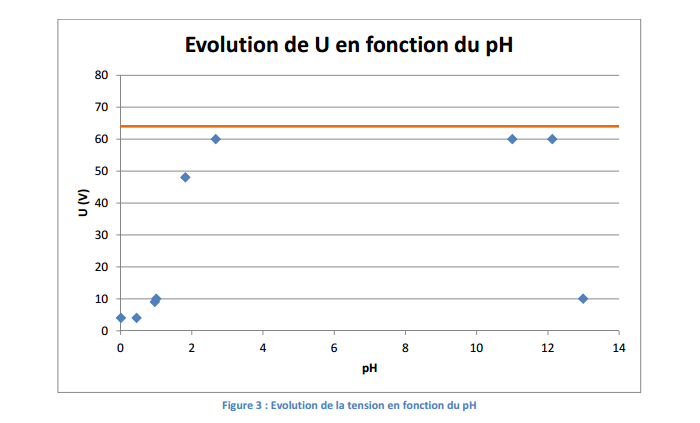
\includegraphics[scale=0.6]{poi.png} 


La variation du pH n'influence pas à priori la vitesse de production de l'hydrogène. Cependant, pour obtenir un même courant à des pH différents, il fallait ajuster la tension (V). A certains pH, il était même impossible d'obtenir un courant de \unit{0.5}{A} à cause de la tension limitée que pouvait produire notre générateur (\unit{64}{V} maximum). Il est donc important de bien ajuster l'acidité du milieu en fonction du générateur à disposition. On remarque donc que le pH influence bien la production d'hydrogène car une augmentation de la tension implique une augmentation de la puissance. Cependant, l'électrolyse peut se réaliser sans apport de changement de pH. Il est  préférable économiquement de réaliser cette expérience à pH neutre car le modifier suggère d'importer des réactifs supplémentaires en grande quantité bien qu'il faille imposer une puissance plus intense. 

\section{Puissance requise pour un flux d'hydrogène}

Pour produire \unit{1500}{t/j} d'ammoniac, il faut disposer d'un flux d'hydrogène de \unit{1529.1}{mol/s}. Nous supposerons que le rendement est de \unit{100}{\%} et que la réaction se déroule dans les conditions standard. 

La réaction de l’électrolyse de l'eau est la suivante : 
$$\ce {2H2O(l) -> 2H2(g) + O2(g)}$$ 

Calculons l'enthalpie molaire de réaction :

$$ \Delta H_r^0 =  \unit{285}{kJ.mol^{-1}} $$

La puissance (P) à fournir au système est simplement le produit du flux d'hydrogène exigé et de $ \Delta H_r^0$ :

$$ P = 285\cdot1529.1 = \unit{435 793.5}{kW} $$



\end{document}
